\documentclass{article}


\usepackage{arxiv}

\usepackage{placeins}
\usepackage[utf8]{inputenc} % allow utf-8 input
\usepackage[T1]{fontenc}    % use 8-bit T1 fonts
\usepackage{hyperref}       % hyperlinks
\usepackage{url}            % simple URL typesetting
\usepackage{booktabs}       % professional-quality tables
\usepackage{amsfonts}       % blackboard math symbols
\usepackage{nicefrac}       % compact symbols for 1/2, etc.
\usepackage{microtype}      % microtypography

\usepackage{graphicx}	% to insert graphs
\usepackage{caption}	% to customize caption style
\usepackage{float}
\usepackage{subfigure}



\title{COMP0037 ASSIGNMENT 2}


\author{
 Group: \texttt{Group L}\\
}

\date{}

\begin{document}

\maketitle

\captionsetup[figure]{labelformat={default},labelsep=period,name={Fig.}}


% -------------------------------------------------------------------------------------------
\section{Introduction [dai ding]} 

% -------------------------------------------------------------------------------------------
\section{Reactive Planner [Yun]}
% -----------
\subsection {Reactive Planning System}

A reactive planning system works like that: The planner makes a trajectory using the latest world model and the free space assumption. And the robot constantly perceives the environment and updates the world map as it moves. When the original path has become blocked by an obstacle, it reacts by planning a new set of actions and plans. See the block diagram in Fig. \ref {fig:reactivePlanningSystem}.

\begin{figure}[ht]
\centering
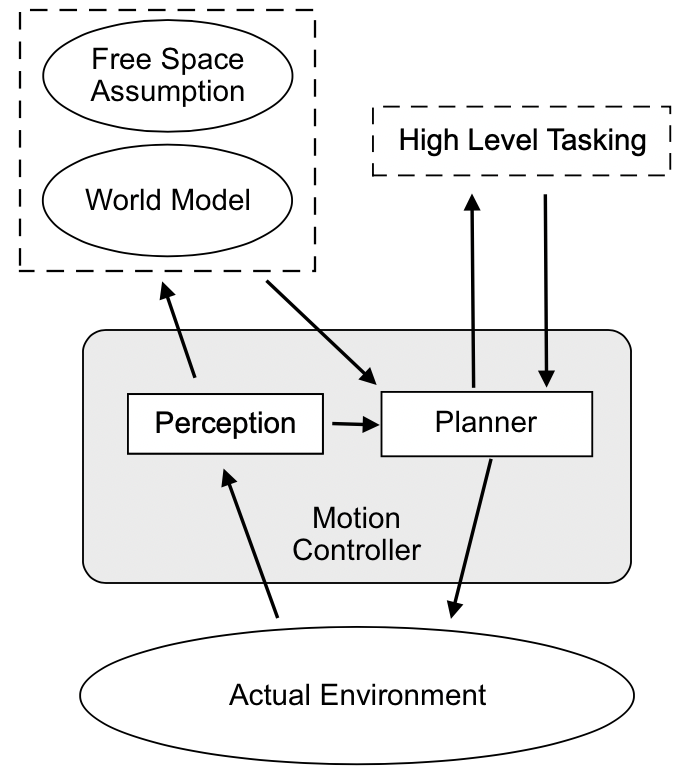
\includegraphics[scale=0.5]{graphs/part1/reactivePlanningSystem.PNG}
\caption{Reactive Planning System}
\label{fig:reactivePlanningSystem}
\end{figure}

% -----------
\subsection {Our Implementation}

We implement the reactive planning system by complete the function \textit{checkIfCurrentPathIsStillGood} in the \textit{ReactivePlannerContoller.py}. The code is shown in Fig. \ref{fig:code}.

\begin{figure}[ht]
\centering
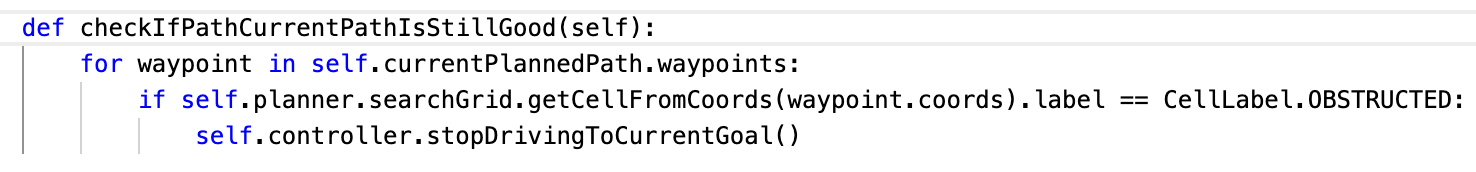
\includegraphics[scale=0.6]{graphs/part1/code.PNG}
\caption{}
\label{fig:code}
\end{figure}

The result is shown in Fig.\ref{fig:result1} and Fig.\ref{fig:result2}.

\begin{figure}[H]
\centering  
\subfigure[STDR GUI]{
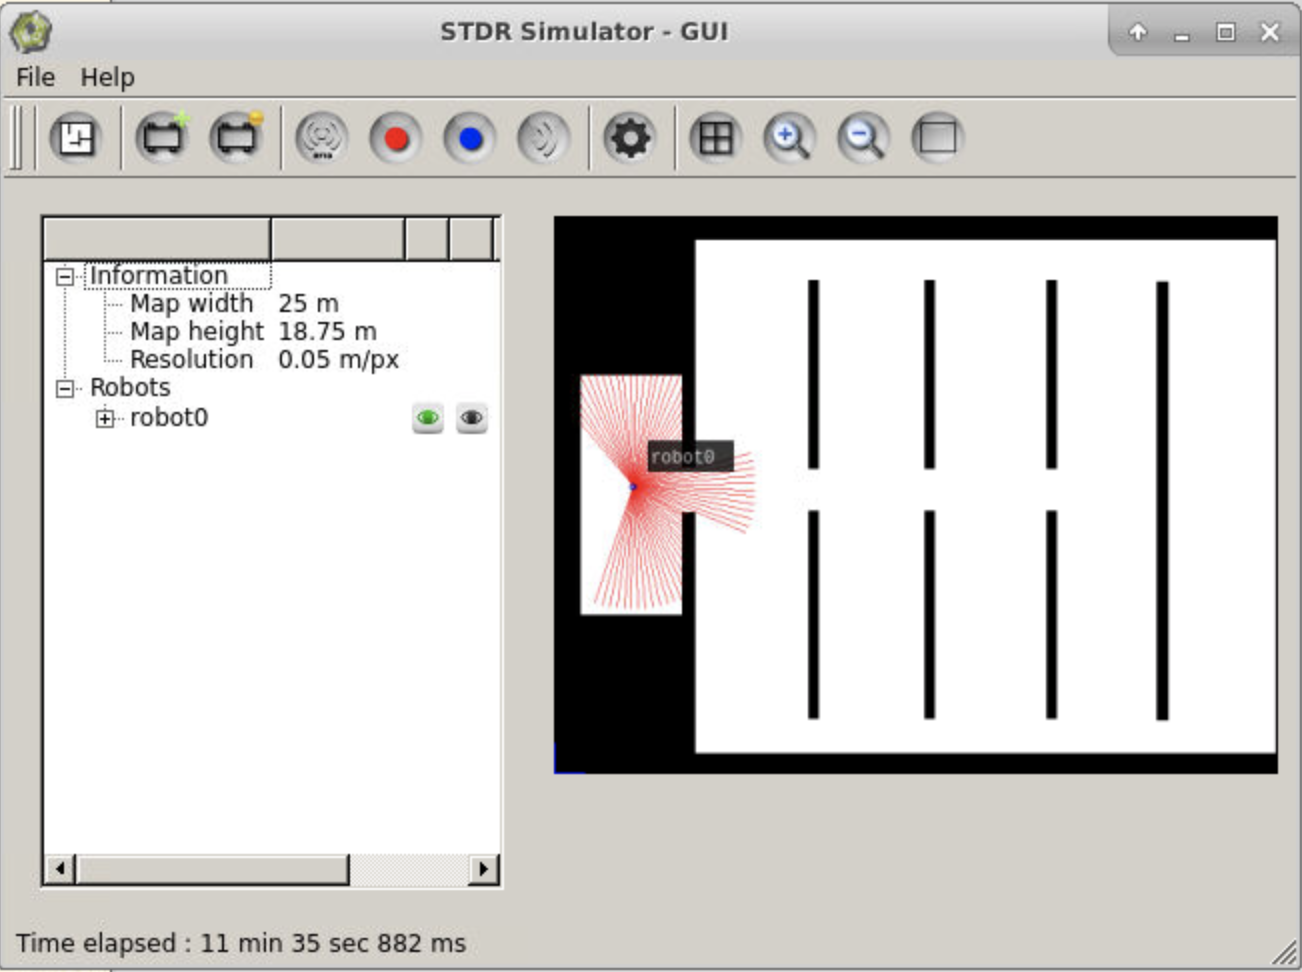
\includegraphics[width=0.45\textwidth]{graphs/part1/1-1/GUI.png}}
\subfigure[Planner Occupancy Grid]{
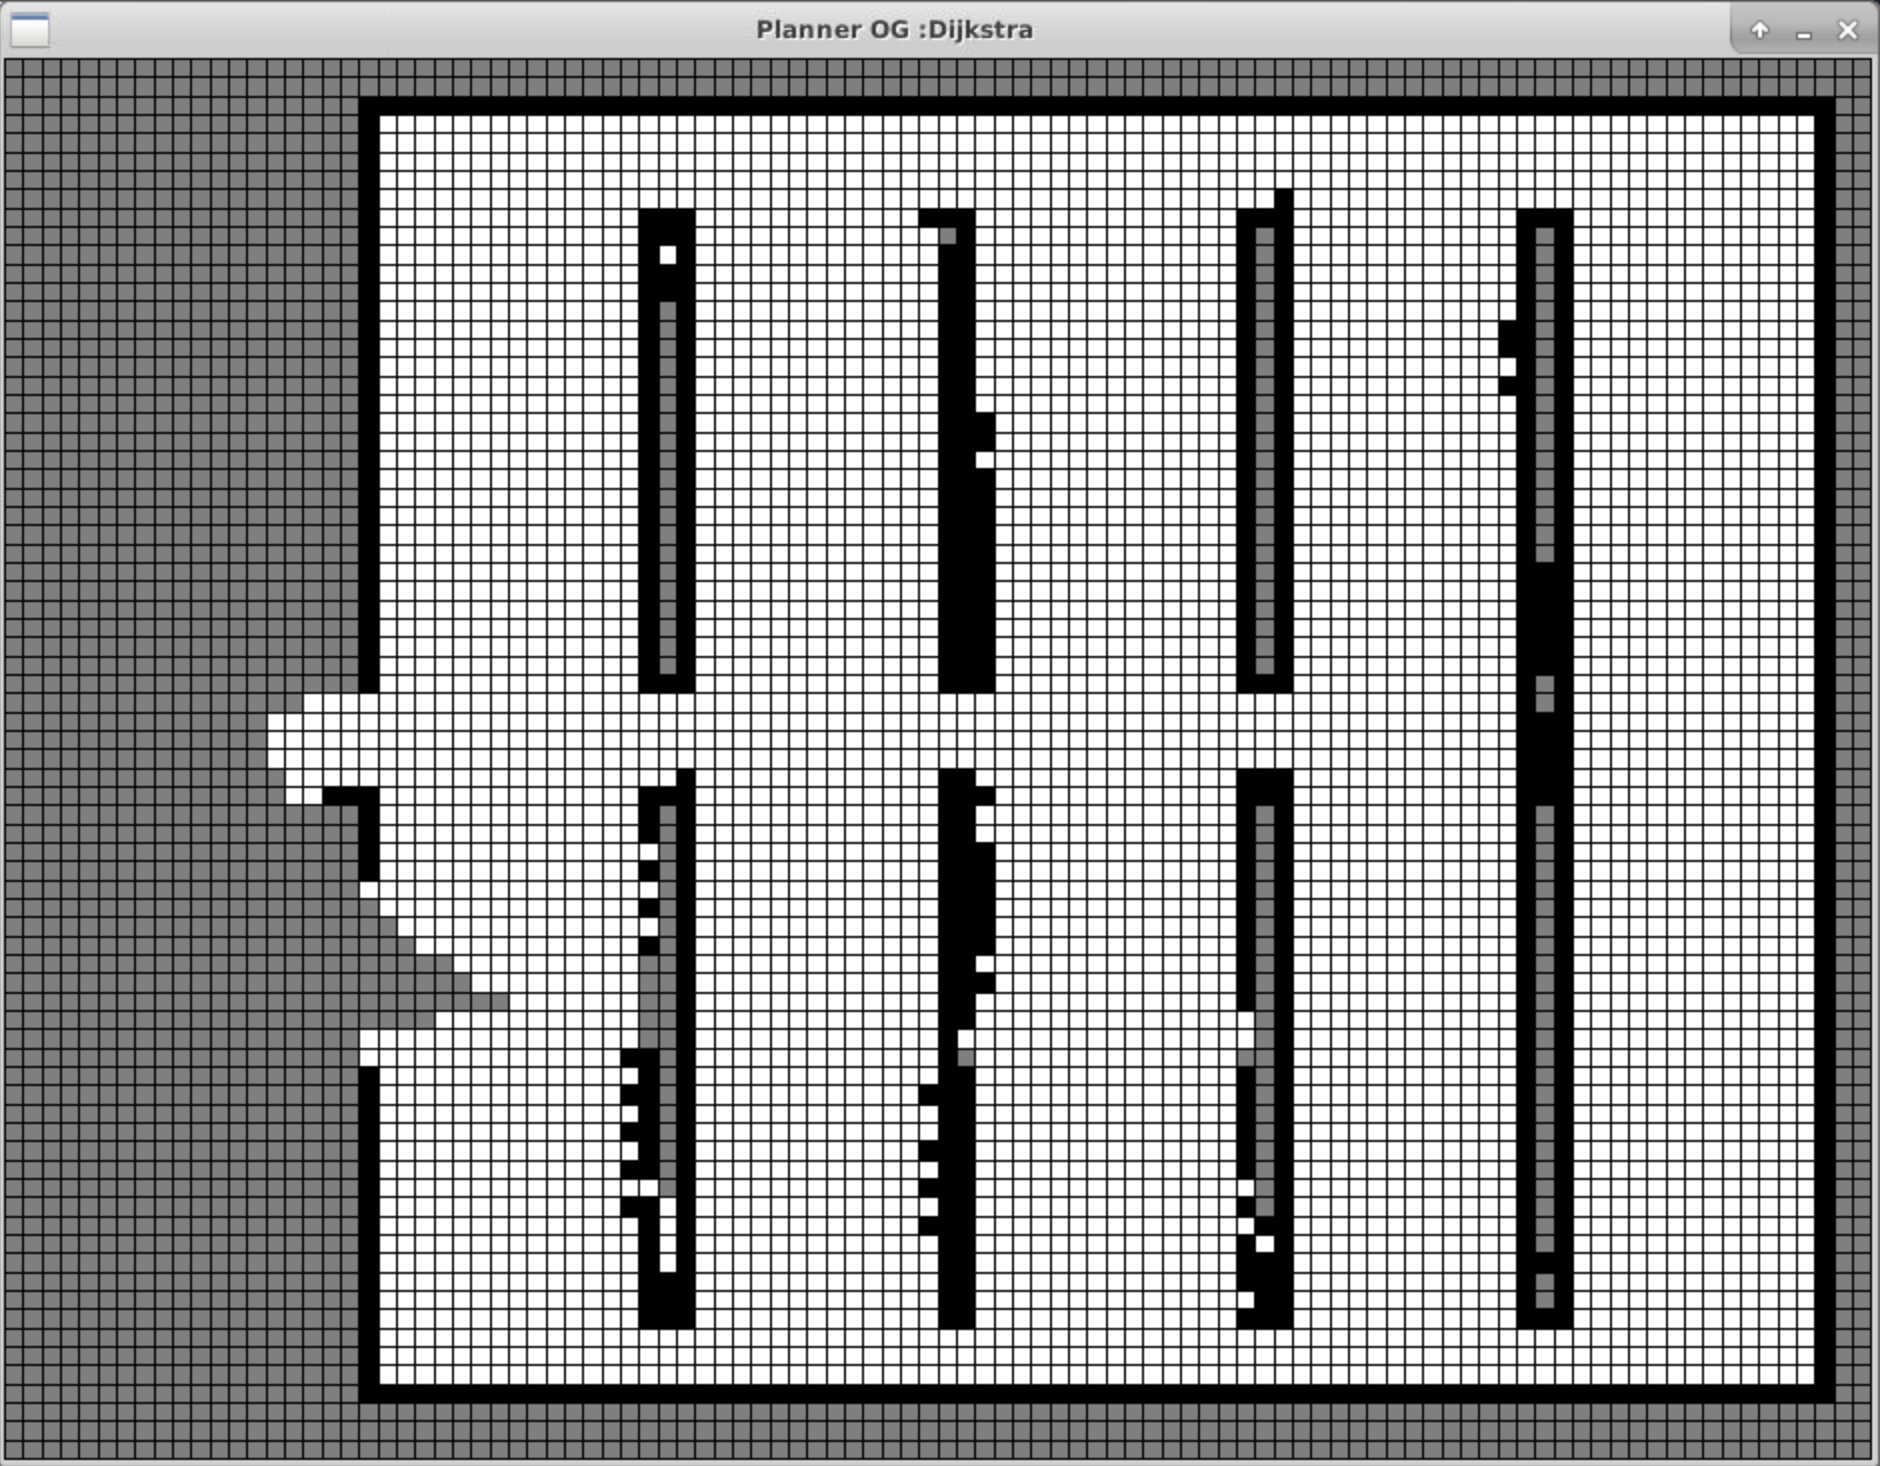
\includegraphics[width=0.45\textwidth]{graphs/part1/1-1/plannerOG.png}}
\subfigure[Planner Search Grid]{
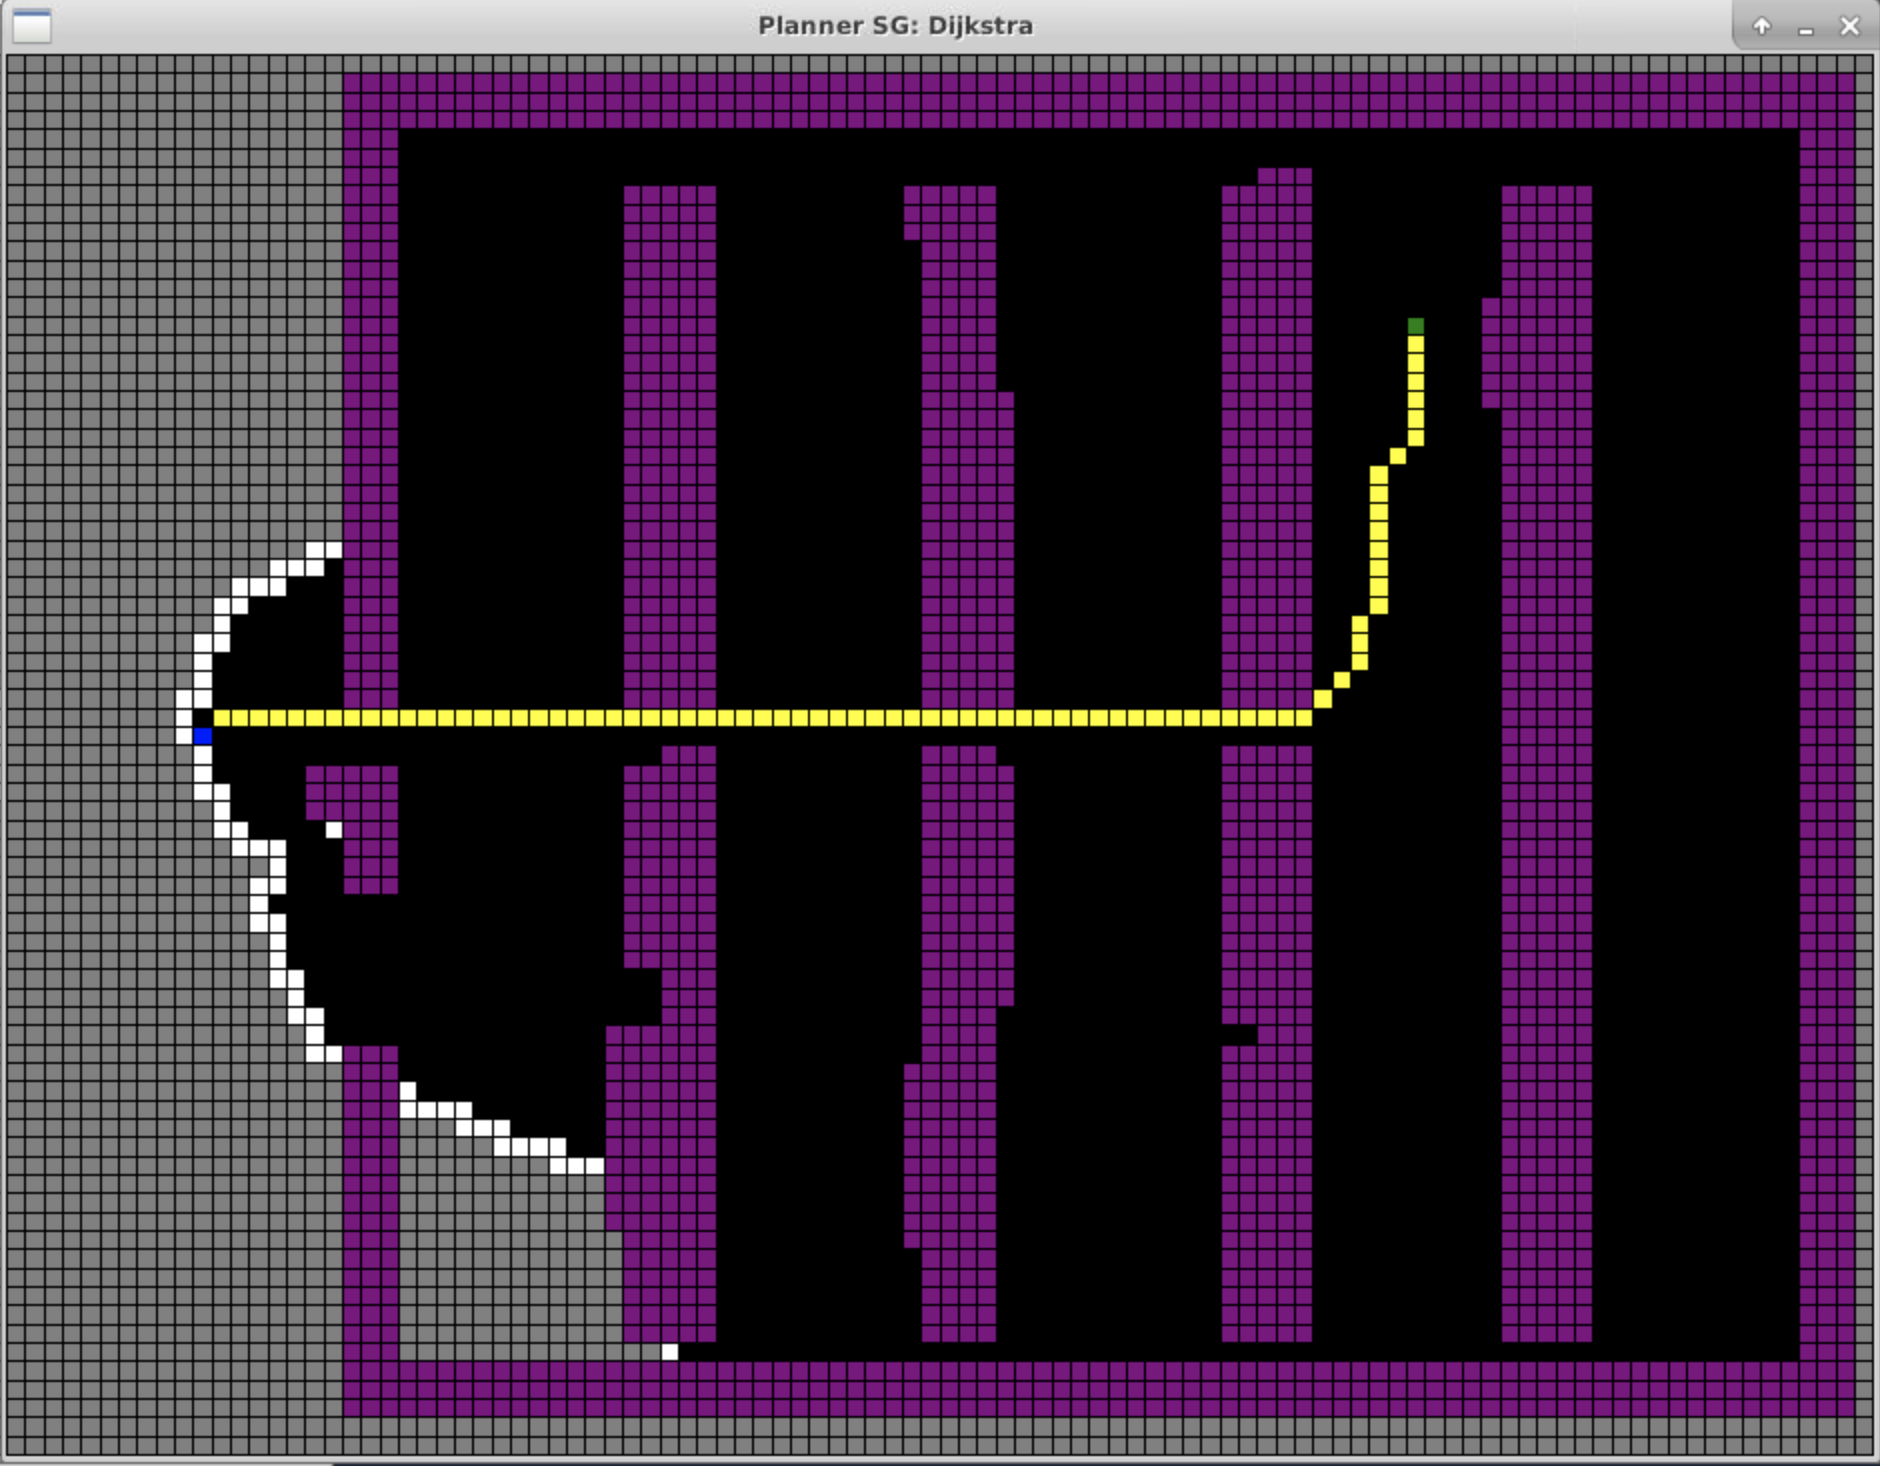
\includegraphics[width=0.45\textwidth]{graphs/part1/1-1/plannerSG.png}}
\subfigure[Mapper Node Occupancy Grid]{
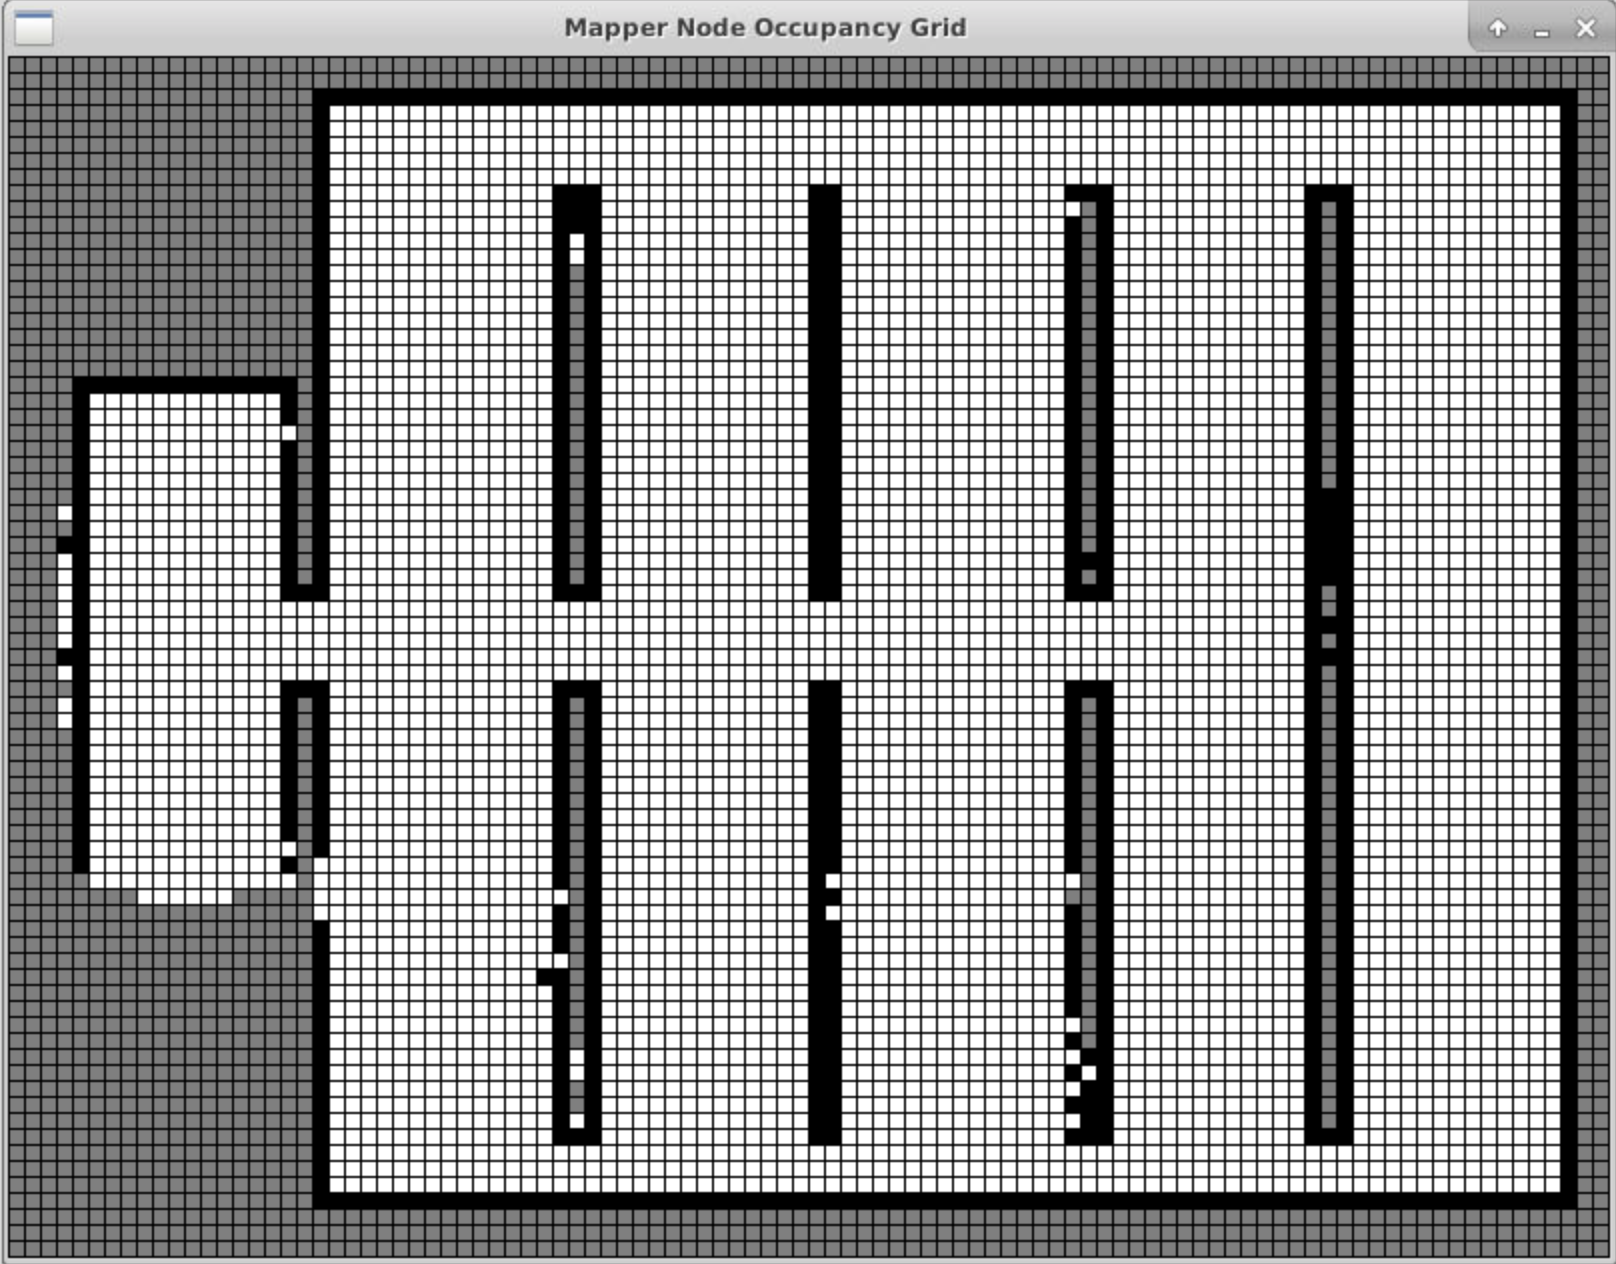
\includegraphics[width=0.45\textwidth]{graphs/part1/1-1/mapperNodeOG.png}}
\caption{Result on the first launch script}
\label{fig:result1}
\end{figure}

\begin{figure}[H]
\centering  
\subfigure[STDR GUI]{
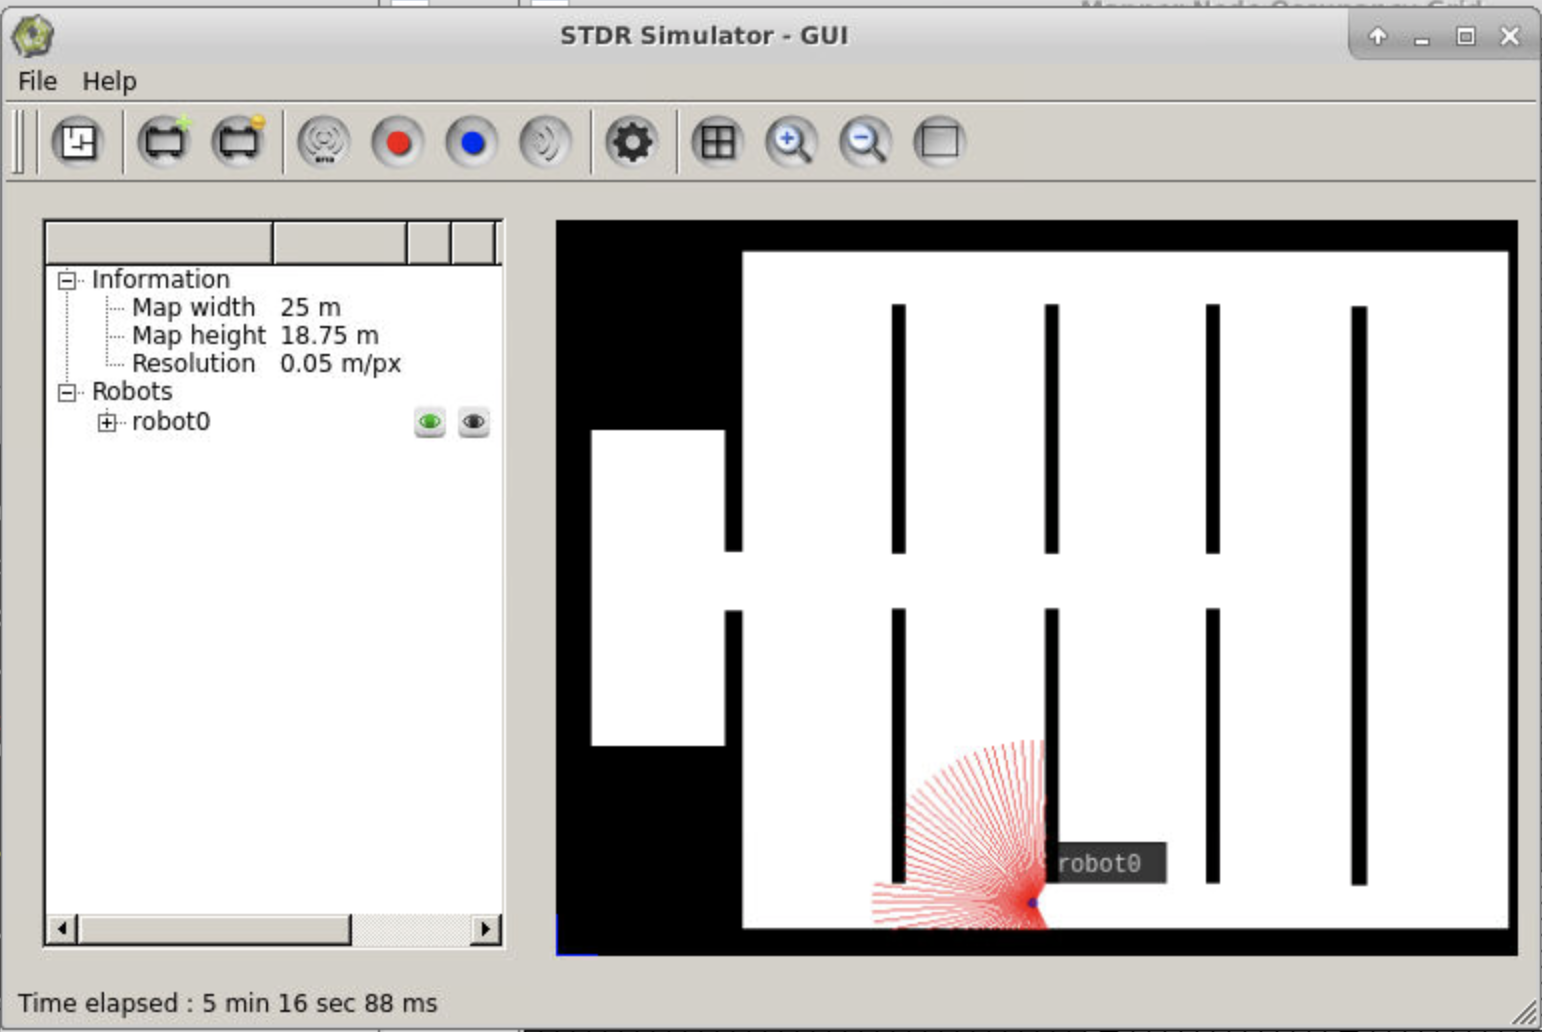
\includegraphics[width=0.45\textwidth]{graphs/part1/1-2/GUI.png}}
\subfigure[Planner Occupancy Grid]{
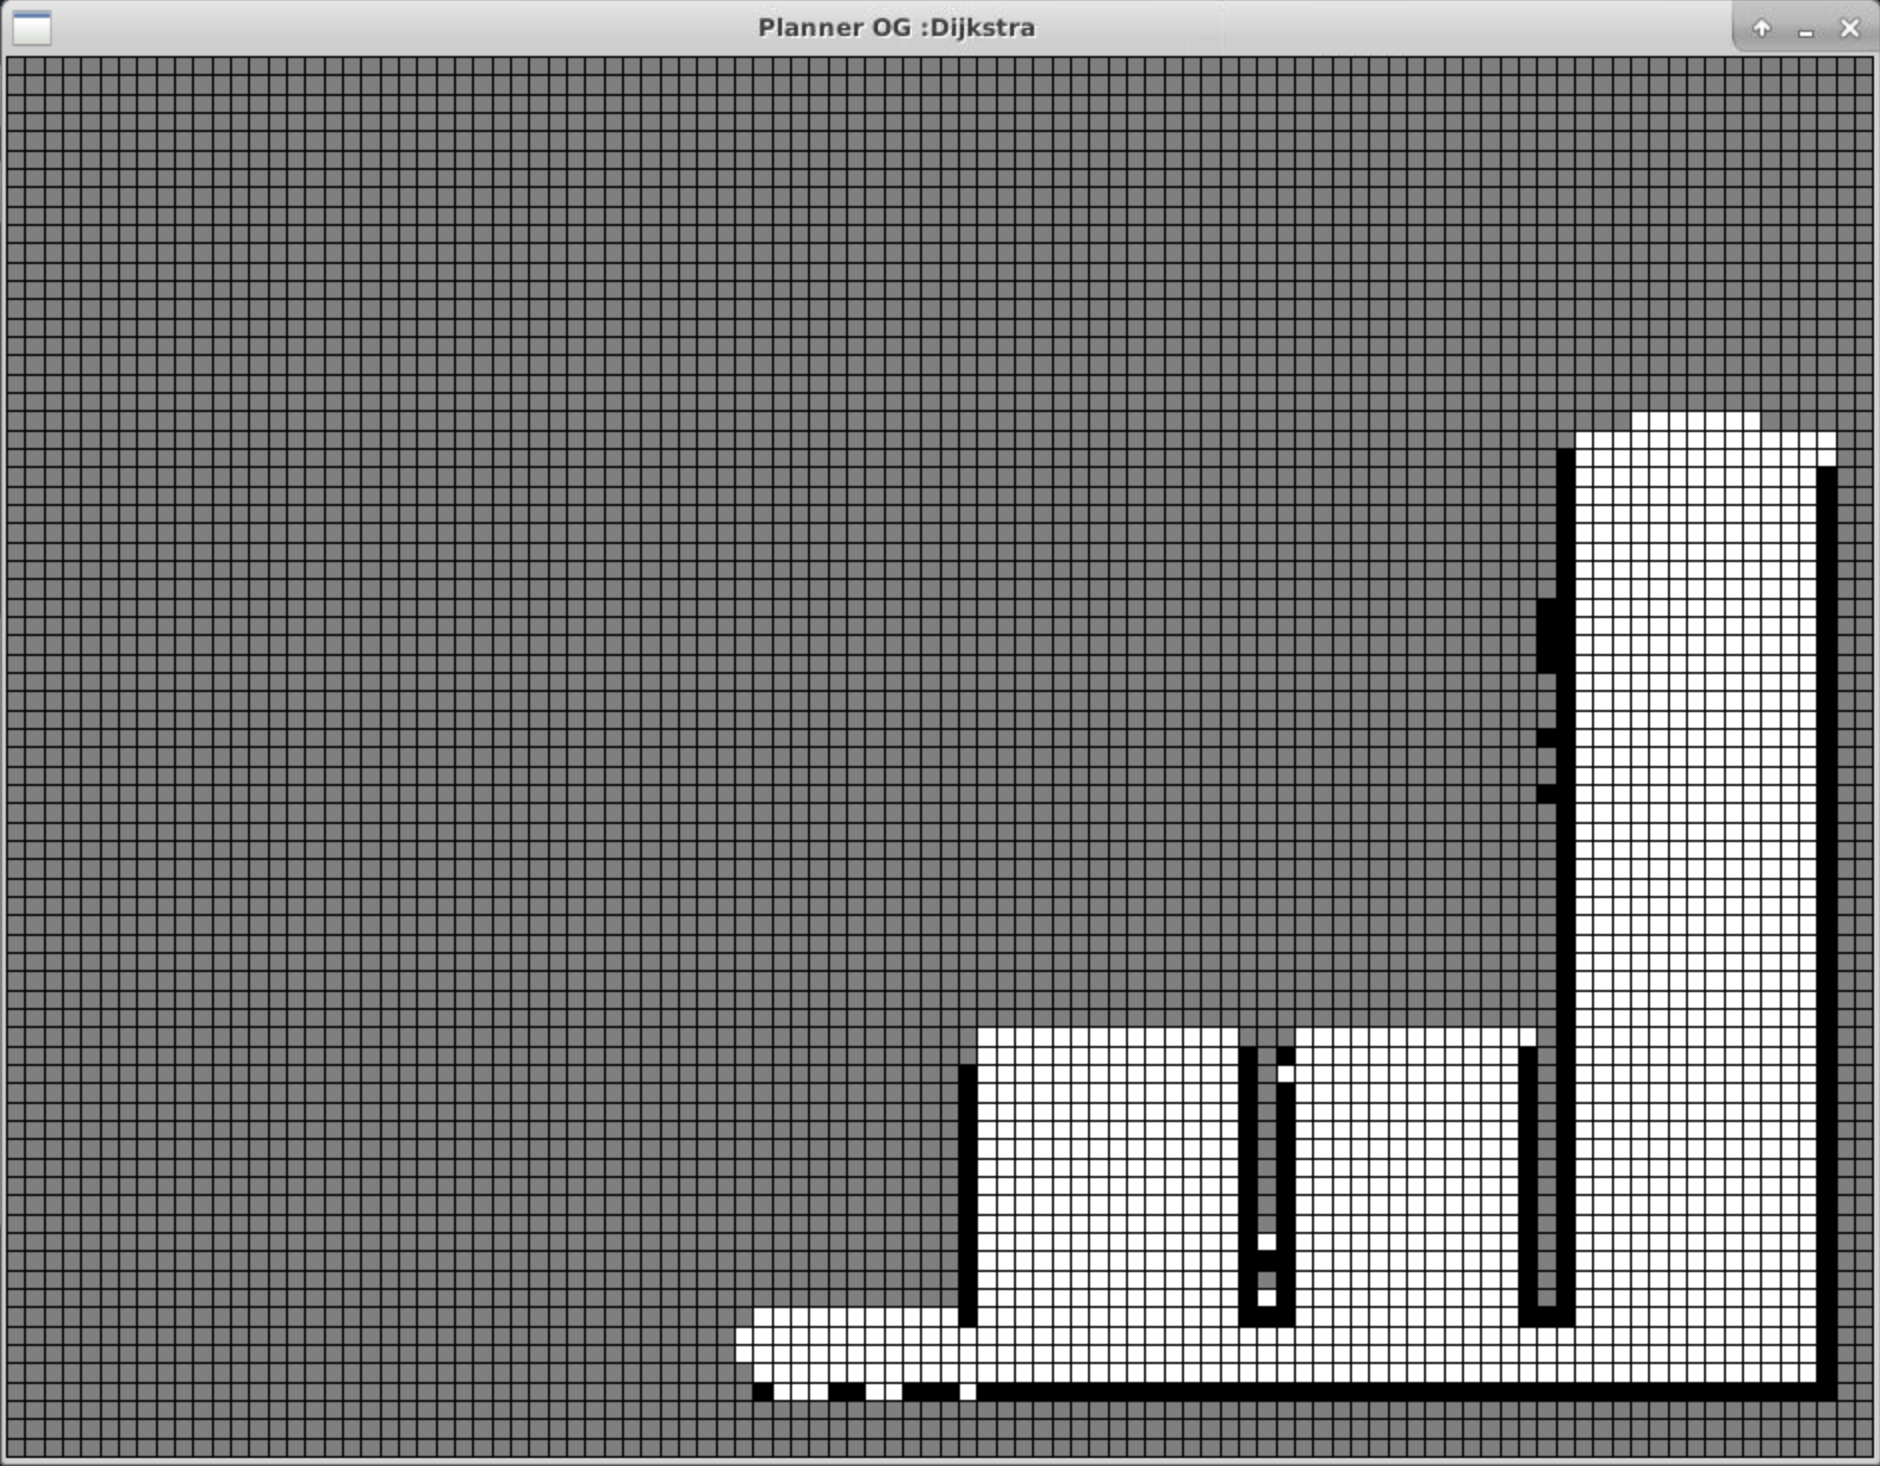
\includegraphics[width=0.45\textwidth]{graphs/part1/1-2/plannerOG.png}}
\subfigure[Planner Search Grid]{
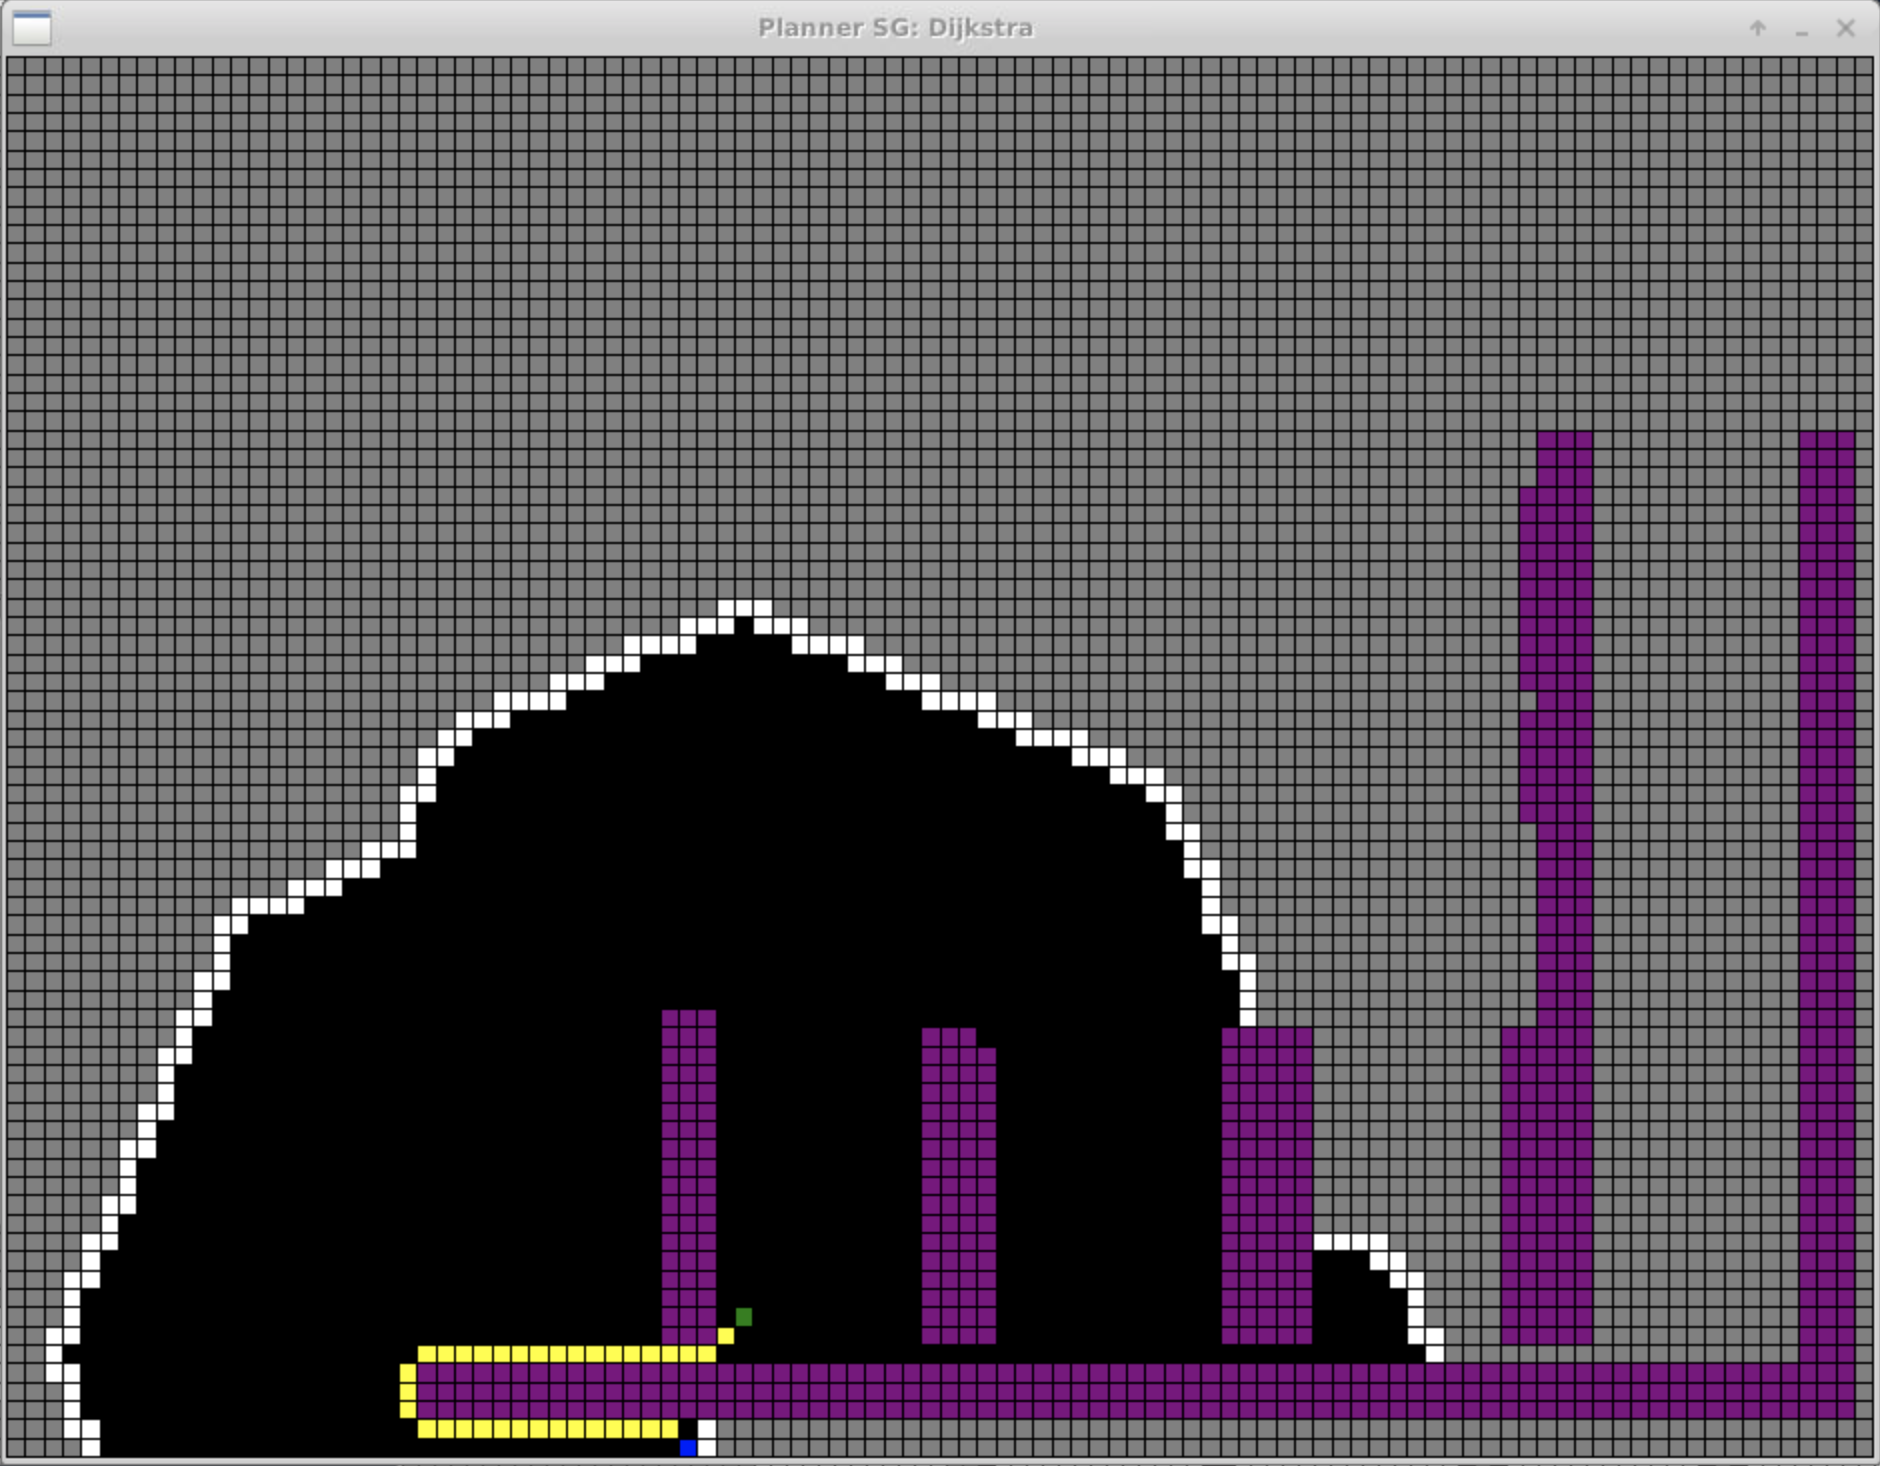
\includegraphics[width=0.45\textwidth]{graphs/part1/1-2/plannerSG.png}}
\subfigure[Mapper Node Occupancy Grid]{
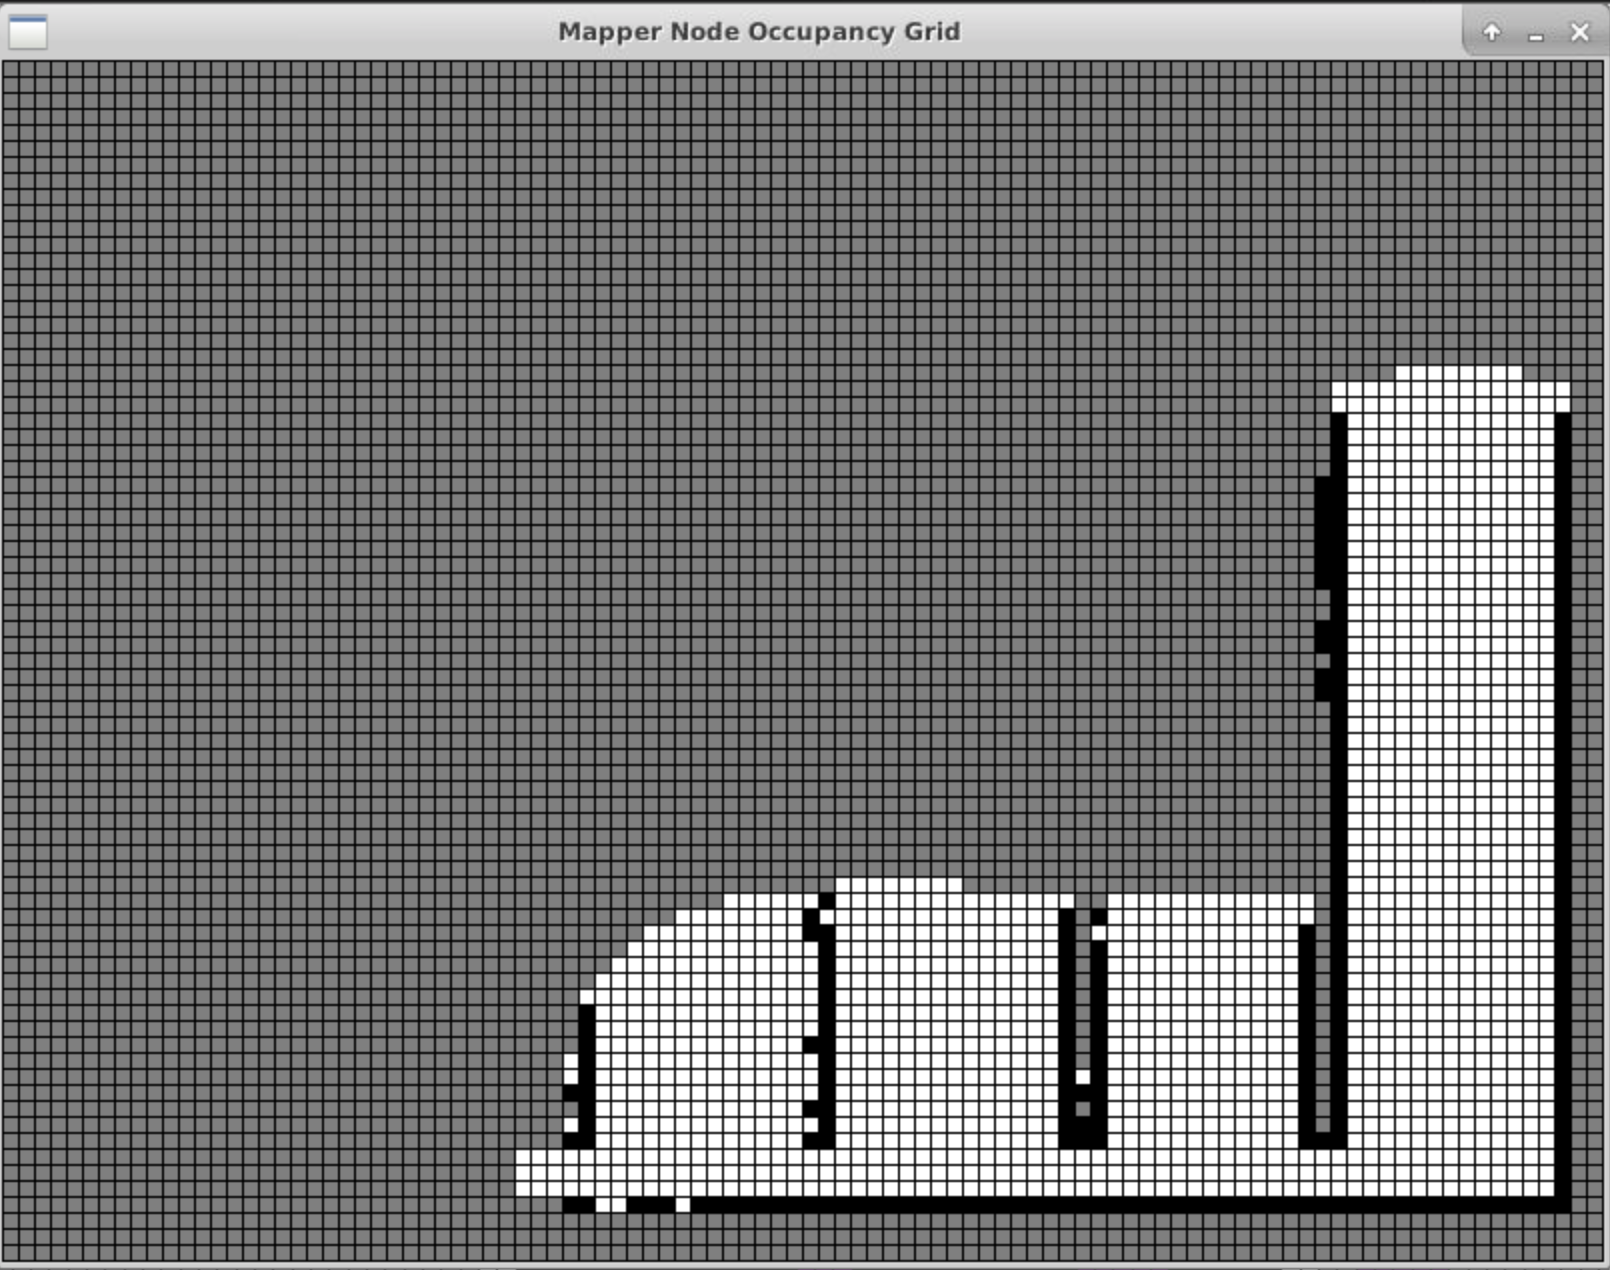
\includegraphics[width=0.45\textwidth]{graphs/part1/1-2/mapperNodeOG.png}}
\caption{Result on the second launch script}
\label{fig:result2}
\end{figure}

% -----------
\subsection {Approach for Improving the Performance}

One approach for improving the performance is using a more efficient global planner to reduce the computational cost associated with re-planning. D*-Lite is one such algorithm that caches previous searches and update them only when we need to. It make use of the backwards search. The graph additionally contains a consistency condition. When the graph changes, such as due to an obstacle, the consistency condition is violated. A priority queue is then used to sort the effect of the failed condition on the path. The highest priority updates are committed first.


% -------------------------------------------------------------------------------------------
\section{Frontier-Based Exploration System [Yun]}

\subsection {Frontiers}

A frontier is a cell which its state is known while it is adjacent to a cell whose state is not known. Frontier cells define boundary between open space and the uncharted territory. In frontier-based exploration, the robot moves to the boundary to gain the newest information about the world.

Two methods for identifying frontiers are wave front detection and fast frontier detection.The wave front detection explores the map based on the map that has already been explored. It searches the frontiers using depth-first search, starting from the robot initial location. Once a cell is encountered that looks like a frontier, it pauses the search and traces along all the frontier cells. The latter relies on the newly collected sensor information. The sensor data is used to create a contour, which then be separated into frontier and non-frontier segments. The frontier segments are managed in a database to make them persistent. When data becomes available, the frontiers will be split or merged deleted. One heuristic for choosing next waypoint is picking the closest frontier to the robot. Another one is picking the largest frontier cell.


\subsection {The Exploration Algorithm Provided}

\subsection {Our Implementation}

% -------------------------------------------------------------------------------------------
\section{Integration of Our Planner and Exploration System [Yun]}

% -------------------------------------------------------------------------------------------
\section{Information-Theoretic Path Planning [Yusi]}

% -------------------------------------------------------------------------------------------
\section{Conclusion [dai ding]}

% -------------------------------------------------------------------------------------------
\bibliographystyle{unsrt}  
%\bibliography{references}  %%% Remove comment to use the external .bib file (using bibtex).
%%% and comment out the ``thebibliography'' section.


%%% Comment out this section when you \bibliography{references} is enabled.
\begin{thebibliography}{1}

\end{thebibliography}


% -----------------------------------------------------------------------------------------
\end{document}